\documentclass[11pt,a4paper]{article}
\usepackage[T1]{fontenc}
\usepackage[utf8]{inputenc}
\usepackage{lmodern,microtype}
\usepackage[margin=25mm]{geometry}
\usepackage{amsmath,amssymb,amsthm,mathtools}
\usepackage{graphicx,booktabs,array}
\usepackage[numbers,sort&compress]{natbib}
\usepackage[colorlinks=true,allcolors=blue,breaklinks=true]{hyperref}
\usepackage{url}
\hypersetup{pdftitle={A second-order obstruction to localized edge-mode continuation in a non-Hermitian interacting Kitaev chain},pdfauthor={Xiaojian Zeng}}
\newcommand{\ii}{\mathrm{i}}
\newcommand{\Id}{\mathbf{1}}
\newcommand{\ad}{\operatorname{ad}}
\newcommand{\Ran}{\operatorname{Ran}}
\newcommand{\diag}{\operatorname{diag}}
\newcommand{\cond}{\operatorname{cond}}
\newcommand{\Rea}{\operatorname{Re}}
\newcommand{\Ima}{\operatorname{Im}}
\newcommand{\norm}[1]{\left\lVert#1\right\rVert}
\newtheorem{proposition}{Proposition}
\newtheorem{lemma}{Lemma}
\setlength{\emergencystretch}{2em}
\title{A second-order obstruction to localized edge-mode continuation\newline
in a non-Hermitian interacting Kitaev chain}
\author{Xiaojian Zeng\\[3pt]
\small PBC School of Finance, Tsinghua University, 100190\\
\small\texttt{xiaojianzeng@foxmail.com}}
\date{}
\begin{document}
\maketitle
\begin{abstract}
An edge commutator zero mode on an exactly solvable slice need not admit a smooth
localized continuation away from that slice. We establish a controlled example
in the dimerized non-Hermitian interacting Kitaev chain with its physical open
left boundary. At $U/t=\delta/t=\eta=1/5$, $\mu=0$, and
$\Delta/t=1+\epsilon$, the normalized edge operator at $\epsilon=0$ has a
unique parity-odd exponentially localized first-order correction. A
five-mode continuum resonance nevertheless obstructs every exponentially
localized second-order correction. The argument combines a bounded
half-line spectral similarity, uniqueness across all Clifford degrees, and
a nonzero on-shell forcing functional. An exact dyadic finite witness,
checked with ball arithmetic and a weighted inverse estimate, gives
$0.0001054530<\Rea\Phi/t<0.0001525309$ for the infinite half-line
forcing in the specified scattering normalization. The error includes the
physical bond crossing the witness cutoff and the complete omitted source
tail. A separately generated witness also excludes zero. The obstruction
persists despite positive one-particle real-line gaps and a regular first-order
correction. It excludes the stated twice-differentiable local continuation;
it does not determine a finite-perturbation phase boundary or exceptional point,
or exclude nonanalytic branches and branches with nonlocal derivatives.
\end{abstract}

\section{Introduction}
Exact strong zero modes in interacting chains provide a stringent form of
boundary-operator structure. Fendley's construction for the uniform XYZ chain
shows that such structure can survive interactions~\cite{Fendley2016}. Its
survival under changes of the Hamiltonian, however, depends on more than the
existence of a localized mode in an unperturbed quadratic representation.
Perturbative resonances and overlapping excitation bands already play a
central role in the stability of boundary strong zero modes in other
models~\cite{Olund2025}. A vanishing perturbative denominator alone is
insufficient to decide continuation: the forcing can vanish on the resonant
channel, and homogeneous solutions can change the next-order equation.

We study the non-Hermitian interacting Kitaev model of Sayyad and
Lado~\cite{Sayyad2023}. Their exactly solvable slice has equal hopping and
pairing, zero chemical potential, and common dimerization of the hopping,
pairing, and complex interaction. We vary the pairing away from that slice
at a specified non-Hermitian, dimerized point. The result is a
second-order obstruction for a normalized edge \emph{commutator} operator on
the original half-line. We do not infer a many-body phase boundary from the
operator equation.

The decisive step is a nonzero forcing functional at a real-momentum
$3A-2B$ resonance, where $A$ and $B$ denote the two quadratic Majorana
subchains. We first construct the localized first-order correction and prove
its uniqueness among all parity-odd localized operators. We then bound the
forcing error for the exact infinite solution using a finite dyadic witness.
This removes both the finite-ansatz ambiguity and the uncontrolled
thermodynamic extrapolation that would otherwise limit a resonance test.
The scope is model-specific. Uniform XYZ constructions and the recent
commutant-algebra study of strong zero modes~\cite{Moudgalya2026} are prior work, as is
the general resonance mechanism~\cite{Olund2025}.

\section{Model, boundary and continuation problem}
For open finite chains, write the defining fermionic Hamiltonian as
\begin{align}
 H_L={}&-\sum_{j=1}^{L-1}m_j\left[t(c_j^\dagger c_{j+1}+c_{j+1}^\dagger c_j)
 +\Delta(c_j^\dagger c_{j+1}^\dagger+c_{j+1}c_j)\right]\notag\\
 &+(U-\ii\delta)\sum_{j=1}^{L-1}m_j(2n_j-1)(2n_{j+1}-1)
 -\mu\sum_{j=1}^L(n_j-\tfrac12),\qquad
 m_j=1+(-1)^{j+1}\eta .\label{eq:fermion}
\end{align}
Here $\{c_j,c_k^\dagger\}=\delta_{jk}$, $n_j=c_j^\dagger c_j$, and
$t>0$ sets the energy unit. All four bond parameters have the same
dimerization. The leftmost bond is $1+\eta$, with no boundary modification.
Equation~\eqref{eq:fermion} is the model in Eqs.~(1)--(2) of
Ref.~~\cite{Sayyad2023}. We set $t=1$ in the derivation and restore it in
dimensional statements. Thus $\epsilon=\Delta/t-1$, all operators $Q_j$,
and the cell momenta are dimensionless, whereas frequencies, commutators and
$\Phi$ have energy units. This is a static effective non-Hermitian
Hamiltonian; no dissipative master equation is specified.

At $U=\delta=\eta=1/5$ and $\mu=0$, the Jordan--Wigner spin representation is
\begin{align}
 H(\epsilon)&=H_0+\epsilon V,\label{eq:expansion}\\
 H_0&=\sum_{j\geq1}m_j[-X_jX_{j+1}+g Z_jZ_{j+1}],
 &g&=\frac{1-\ii}{5},\label{eq:h0}\\
 V&=\frac12\sum_{j\geq1}m_j[-X_jX_{j+1}+Y_jY_{j+1}].\label{eq:v}
\end{align}
$X_j,Y_j,Z_j$ are Pauli matrices on the physical site $j$. The infinite
expressions mean local derivations on the half-line spin algebra, rather
than bounded infinite Hamiltonians. We use the notation $[H,Q]$ for the
norm-convergent commutator series on its domain.

An operator $Q$ is exponentially localized at the left end if there are
$C_Q,\kappa_Q>0$ and operators $Q^{[r]}$ supported on sites $1,\ldots,r$
such that
\begin{equation}
 \norm{Q-Q^{[r]}}\leq C_Q e^{-\kappa_Q r}.\label{eq:locality}
\end{equation}
This is locality in the original-spin operator norm. Constants may differ
between coefficients. Physical fermion parity is the automorphism induced
by $\prod_j Z_j$ on finite local operators.

Define Majoranas
\begin{equation}
 \alpha_j=\left(\prod_{k<j}Y_k\right)X_j,
 \qquad \beta_j=-\left(\prod_{k<j}Y_k\right)Z_j,
 \qquad \{\gamma_j,\gamma_k\}=2\delta_{jk}\Id,
 \label{eq:majoranas}
\end{equation}
where the last relation uses a single enumeration of both families. Put
$A_j=\alpha_j$ for odd $j$ and $A_j=\beta_j$ for even $j$; let
$B_j=\beta_j$ for odd $j$ and $B_j=\alpha_j$ for even $j$.
Every $A_j$ is parity odd and every $B_j$ parity even. Set
\begin{equation}
 \rho=\frac{3(1-\ii)}{10},\qquad C=\sqrt{1-\rho^2},\qquad
 Q_0=C\sum_{n\geq0}\rho^n\alpha_{2n+1},\label{eq:q0}
\end{equation}
using the principal square root. Since $|\rho|^2=9/50<1$, the series
converges in operator norm, $Q_0^2=\Id$, and the half-line recurrence gives
$[H_0,Q_0]=0$. No Hermiticity of $Q_0$ is required.

\begin{proposition}\label{prop:main}
For the physical half-line Hamiltonian~\eqref{eq:h0}--\eqref{eq:v}, there is
a unique parity-odd exponentially localized $Q_1$ satisfying
\begin{equation}
 [H_0,Q_1]=-[V,Q_0],\qquad \{Q_0,Q_1\}=0.\label{eq:first}
\end{equation}
There is no exponentially localized $Q_2$ satisfying
\begin{equation}
 [H_0,Q_2]=-[V,Q_1].\label{eq:second}
\end{equation}
Consequently, there is no twice norm-differentiable exact commutator-zero-mode
branch $Q(\epsilon)$ based at $Q_0$, with exponentially localized first two
Taylor coefficients and square normalization to first order.
\end{proposition}

For the last statement we write $Q(\epsilon)=Q_0+\epsilon Q_1+
\epsilon^2Q_2+o(\epsilon^2)$ in norm, so $Q_2=Q''(0)/2$.
The branch is understood to be in the commutator domain at each nearby
$\epsilon$. Section~\ref{sec:contradiction} justifies extracting the
coefficient equations without assuming an infinite Hamiltonian is bounded.

\section{Half-line spectral representation and uniqueness}
\subsection{Bounded similarity}
Let $a=6/5$ and $b=4/5$. Direct Clifford multiplication gives two subchains,
each of the form
\begin{equation}
 H_s=\ii\sum_{n\geq1}(p_s u_n v_n+h_s v_n u_{n+1}),\qquad
 (p_A,h_A)=(ga,b),\quad(p_B,h_B)=(a,gb),\label{eq:subchain}
\end{equation}
where $u_n=A_{2n-1},v_n=A_{2n}$ in $A$, and similarly for $B$.
On coefficient vectors ordered as $(u,v)$, commutation is
\begin{equation}
 K_s=\begin{pmatrix}0&2\ii D_s\\-2\ii D_s^T&0\end{pmatrix},\qquad
 D_s=p_s\Id-h_s S,\qquad (Sf)_n=f_{n-1},\quad f_0=0.\label{eq:k}
\end{equation}
The superscript $T$ denotes the bilinear transpose, not the Hermitian
adjoint. Since $S^TS=\Id$,
\begin{equation}
 G_s=D_s^TD_s=(p_s^2+h_s^2)\Id-p_sh_s(S+S^T).\label{eq:g}
\end{equation}
The real unitary sine transform diagonalizes $S+S^T$, giving the symbol
$G_s(q)=p_s^2+h_s^2-2p_sh_s\cos q$, $0<q<\pi$. Its real part is
strictly positive for both subchains at our parameters. Hence $G_s^{1/2}$
and $G_s^{-1/2}$ are bounded normal multiplication operators, with the
positive-real-part square-root branch.

Set $J_s=D_sG_s^{-1/2}$. Then $J_s^TJ_s=\Id$.
For $B$, $|h_B|<|p_B|$ makes $D_B$ invertible by a Neumann series, so
$J_BJ_B^T=\Id$. For $A$, $D_A$ is bounded below by
$|h_A|-|p_A|>0$ and has closed range of codimension one. Indeed its sole
left-null condition is determined by
\begin{equation}
 q_n=C\rho^{n-1},\quad D_A^Tq=0,\quad q^Tq=1,\qquad
 J_AJ_A^T=\Id-P_0,\quad P_0=qq^T.\label{eq:projector}
\end{equation}
The codimension follows either from the one-step recurrence for $D_Af=y$
or from the index of the unilateral shift. Its range is the bilinear
orthogonal complement of $q$.

The bounded invertible map
\begin{equation}
 \mathcal S_A(c,f,k)=(qc+J_Af,k),\qquad
 \mathcal S_A^{-1}(u,v)=(q^Tu,J_A^Tu,v)\label{eq:similarity}
\end{equation}
separates the discrete zero mode. Use $\mathcal S_B(f,k)=(J_Bf,k)$
for $B$. On the continuum coordinates the transformed matrix is
$\bigl(\begin{smallmatrix}0&2\ii\sqrt G\\-2\ii\sqrt G&0\end{smallmatrix}\bigr)$.
The constant orthonormal eigenvectors $(\ii,1)/\sqrt2$ and
$(-\ii,1)/\sqrt2$ give signed frequencies
\begin{equation}
 \pm\omega_s(q),\qquad \omega_s(q)=2\sqrt{G_s(q)},\quad
 \Rea\omega_s(q)>0.\label{eq:frequency}
\end{equation}
This is a bounded similarity of the non-Hermitian half-line generator, not
an application of the self-adjoint spectral theorem to $K_s$.

\subsection{All-degree localized kernel}
Clifford monomials are an orthonormal basis of the tracial $L^2$ space of
the half-line spin algebra. Quadratic commutation preserves each degree;
its degree-$k$ action is the additive exterior-power generator of $K_A\oplus
K_B$. The preceding similarities lift to bounded invertible maps at every
fixed degree. A bound uniform in degree is unnecessary.

Every transformed block is multiplication by a sum of independently
variable signed continuum frequencies, with at most one discrete $A$ zero
factor. Any sum containing a continuum variable is a nonconstant analytic
function of that variable because $g\ne0$. Its zero set has product measure
zero, by one-variable analyticity and Fubini's theorem. Coincident momenta
with opposite frequencies do not yield $L^2$ zero vectors: such vectors
would have to be supported on a measure-zero diagonal. The exterior
construction therefore introduces no additional point kernel.

The only parity-odd tracial $L^2$ kernel vector is a multiple of $Q_0$.
An operator satisfying~\eqref{eq:locality} belongs to this $L^2$ space.
Thus the difference of any two parity-odd localized solutions of the first
equation in~\eqref{eq:first} is $cQ_0$. The normalization equation gives
$2c\Id=0$. In particular, arbitrary unforced cubic and higher-degree
homogeneous additions have been excluded, rather than set to zero by an
ansatz.
Without a parity restriction the only additional localized kernel vector
is the degree-zero identity. A homogeneous term $c\Id+dQ_0$ has
anticommutator $2cQ_0+2d\Id$ with $Q_0$, so square normalization removes
both terms. Thus the continuation consequence does not hide a parity
assumption on its first derivative.

\section{Existence and control of the first-order correction}
The perturbation has quadratic and quartic parts. In the physical-site
$A$-before-$B$ ordering,
\begin{align}
 V_2&=\frac{\ii}{2}\left(\sum_{j\ \text{odd}}m_j B_jB_{j+1}
                 +\sum_{j\ \text{even}}m_j A_jA_{j+1}\right),\notag\\
 V_4&=-\frac12\sum_{j\geq1}m_j A_jA_{j+1}B_jB_{j+1}.\label{eq:v4}
\end{align}
Consequently $-[V,Q_0]$ contains only linear $A$ and cubic $AB^2$ terms.
The linear solution follows by differentiating the free edge mode under
$t\mapsto t(1+\epsilon/2)$:
\begin{equation}
 Q_{1,\mathrm{lin}}=
 C\sum_{n\geq0}\rho^n
 \left[\frac{\rho^2}{2(1-\rho^2)}-\frac n2\right]\alpha_{2n+1}.
 \label{eq:linear}
\end{equation}
It is exponentially localized and normalized by differentiation of
$Q_0^2=\Id$. Only the cubic correction can contribute to the
second-order $A^3B^2$ forcing.

Let $f=-[V_4,Q_0]$ and let $K_3=K_A+K_B^{(1)}+K_B^{(2)}$ act on
$A\otimes\bigwedge^2B$ coefficients. The identity
$\{Q_0,[V_4,Q_0]\}=[V_4,Q_0^2]=0$ gives $P_{0,A}f=0$.
Introduce the auxiliary inverse
\begin{equation}
 \widetilde K=K_3+8P_{0,A}.\label{eq:mass}
\end{equation}
The number $8$ has energy units before setting $t=1$. This auxiliary
projector does not change a physical bond or the normalized solution: its
role is to shift the otherwise unbounded inverse in the unforced
zero-$A$ block. Since the shift makes that block invertible,
$P_{0,A}\widetilde K^{-1}f=0$ and $K_3\widetilde K^{-1}f=f$.

The real parts of the positive continuum bands have exact ranges
\begin{equation}
 [A_-,A_+]=[28/25,52/25],\qquad
 [B_-,B_+]=[52/25,68/25].\label{eq:bands}
\end{equation}
For completeness, put $x=-\cos q$. The radicands have positive real part
and $\arg(p_sh_s)=-\pi/4$. Since
$d\omega_s/dx=4p_sh_s/\omega_s$, its real part is positive.
Evaluating the endpoints gives~\eqref{eq:bands}. Direct quadratic
minimization of $|G_s|^2$ also gives
\begin{equation}
 \inf|G_A|=\frac{328}{625\sqrt2},\qquad
 \inf|G_B|=\frac{692}{625}.\label{eq:gmin}
\end{equation}
Every shifted cubic multiplier has modulus at least
\begin{equation}
 d=\min\{A_--(B_+-B_-),\;2B_--A_+,\;8-2B_+\}=\frac{12}{25}.
 \label{eq:gap}
\end{equation}
The three terms cover opposite $B$ signs, equal $B$ signs, and the
shifted discrete $A$ factor, respectively.

Useful conservative bounds are
\begin{align}
 j_s&=\frac{(|p_s|+|h_s|)^2}{\inf|G_s|},\qquad
 q_*^2=\frac{|1-\rho^2|}{1-|\rho|^2},\notag\\
 \cond(\mathcal S_A)&\leq q_*^2+j_A,\qquad
 \cond(\mathcal S_B)\leq j_B,\qquad
 \norm{\widetilde K^{-1}}\leq M=\frac{(q_*^2+j_A)j_B^2}{d}<33.318.
 \label{eq:inverse}
\end{align}
Here $j_A,j_B>1$. Bilinear transposition preserves the operator norm,
which justifies using the same bounds for the inverse maps.

For cubic coefficients define a diagonal weight $W_\alpha$ by
$\exp[\alpha(n_A+n_{B_1}+n_{B_2})]$, where the cell indices start at
zero, and choose $\alpha=1/1000$. Appendix~\ref{app:weight} gives an
explicit bound
\begin{equation}
 \norm{W_\alpha\widetilde K W_\alpha^{-1}-\widetilde K}
 \leq E<0.013647916,\quad ME<0.454721,\quad
 \norm{W_\alpha\widetilde K^{-1}W_\alpha^{-1}}<61.103.
 \label{eq:weighted}
\end{equation}
The conjugated identity is first defined on finite sequences. Its bounded
difference from $\widetilde K$ and the Neumann bound produce a weighted
solution; since $W_\alpha^{-1}$ is bounded, it agrees with the unique
unweighted solution. The geometric source belongs to the weighted space.
Cauchy--Schwarz with a smaller positive weight converts weighted coefficient
$\ell^2$ summability at fixed degree into absolute coefficient summability
and an exponential operator-norm tail. Therefore
$Q_{1,\mathrm{cub}}=\widetilde K^{-1}f$ has the locality in
Eq.~\eqref{eq:locality}. Together with~\eqref{eq:linear} and the
all-degree kernel argument, this proves the first assertion of
Proposition~\ref{prop:main}.

\section{A nonzero resonant second-order forcing}
\subsection{Half-line left rows and the exact resonance}
For an interior momentum $q$ and either signed frequency $\omega$, define
the bilinear left scattering row
\begin{equation}
 \ell_{v,n}=\sin(nq),\qquad
 \ell_{u,n}=-\frac{2\ii}{\omega}
       [p\sin(nq)-h\sin((n-1)q)].\label{eq:rows}
\end{equation}
Both column recurrences give $\ell K=\omega\ell$. At the open end
$\sin(0q)=0$ enforces the original boundary. The rows are bounded and,
in $A$, annihilate the discrete mode since $p-h\rho=0$.

Use three positive $A$ rows and two negative $B$ rows at momenta specified
by $x=-\cos q$:
\begin{equation}
 x_{A,1}=-99/100,\quad x_{A,2}=-95/100,\quad x_{A,3}=x,
 \qquad x_{B,1}=y-1/100,\quad x_{B,2}=y+1/100.\label{eq:momenta}
\end{equation}
There is an exact root of
\begin{equation}
 \Omega(x,y)=\sum_{r=1}^3\omega_A(q_{A,r})
                    -\sum_{s=1}^2\omega_B(q_{B,s})=0\label{eq:resonance}
\end{equation}
in the real two-coordinate box of radius $10^{-20}$ centered near
$(0.914006,-0.769582)$.
The full exact decimal center and a contraction certificate are given in
Appendix~\ref{app:root}. The root is established by a self-map contraction,
not by a small residual or by an interval that merely contains zero.
All five momenta are interior, and all radicands retain positive real part
throughout the box.

For increasing physical $A$ indices $i_1<i_2<i_3$ and $B$ indices $j_1<j_2$,
define $\ell_5$ on $A_{i_1}A_{i_2}A_{i_3}B_{j_1}B_{j_2}$ as
\begin{equation}
 \ell_5(A_{i_1}A_{i_2}A_{i_3}B_{j_1}B_{j_2})
 =\det[\ell^A_r(i_s)]_{r,s=1}^3\,
  \det[\ell^B_r(j_s)]_{r,s=1}^2.\label{eq:ell5}
\end{equation}
The $B$ rows use the negative frequencies in~\eqref{eq:rows}.
This fixes the normalization of the forcing functional
\begin{equation}
 \Phi(X)=\ell_5\bigl([V_4,X]_{A^3B^2}\bigr),\qquad X\in AB^2.
 \label{eq:phi}
\end{equation}
Its complex value depends on the row normalization. Its nonvanishing is
unchanged by any nonzero rescaling of those rows. It is not a decay rate.

\subsection{A posteriori bound for the infinite solution}
Let $X$ be a finite cubic coefficient vector extended by zero onto the
physical half-line. Put $R=f-\widetilde KX$. The inverse estimate and a
weighted dual bound on $\Phi$ give
\begin{equation}
 |\Phi(Q_{1,\mathrm{cub}})-\Phi(X)|
 \leq 1248632935\,\norm{W_\alpha R}_2.\label{eq:error}
\end{equation}
The constant is dimensionless; dividing both sides and the residual by $t$
restores the same inequality at general energy units. To obtain it, each
of the two $B$ indices of a cubic monomial can overlap at most two quartic
bonds. If
\begin{equation}
 m_A=\max\{1,2(|p_A|+|h_A|)/A_-\},\quad
 m_B=\max\{1,2(|p_B|+|h_B|)/B_-\},\label{eq:rowbound}
\end{equation}
the determinant estimates $6m_A^3$ and $2m_B^2$ imply
\begin{equation}
 \norm{\Phi W_\alpha^{-1}}
 \leq (4a)(6m_A^3)(2m_B^2)
           \frac{2}{(1-e^{-2\alpha})^{3/2}}
 <20435046.\label{eq:dual}
\end{equation}
There are two coordinates per cell in each species; the exterior $B^2$
sum is at most half the full tensor sum. The product of the unrounded
weighted inverse and dual bounds is less than $1248632935$.
The rounded bounds displayed separately in~\eqref{eq:weighted} and
\eqref{eq:dual} are not used to take that product.

The primary witness has $L=96$ physical sites in its finite generator:
$95$ $A$ coordinates and $96$ $B$ coordinates. These are support cutoffs,
not modified half-line equations. Its stored binary floating-point
coefficients are interpreted as exact dyadic rationals. The certificate
reconstructs the quadratic action with Gaussian integers and rational
couplings, then encloses the geometric source and $C$ with 224-bit Arb
ball arithmetic~\cite{Johansson2017}. It does not trust the finite solver's
eigenvectors, residual estimates, or convergence claim.

The residual includes the physical $A$ link across the cutoff, the $B$
link across the cutoff, the normalization term $8P_{0,A}X$, and the
entire omitted geometric source. For $N=L/2$, the latter has the
conservative bound
\begin{equation}
 T_N=\frac{4a|C|e^{3\alpha(N+2)}|\rho|^N}
                  {1-|\rho|e^{3\alpha}}.\label{eq:tail}
\end{equation}
It overcounts the two bonds touching each remaining edge coefficient and
starts early enough to include every unrepresented source entry. Explicit
finite and normalization bounds are in Appendix~\ref{app:residual}.

\begin{table}[tb]
\centering
\caption{Certified error budget for the $96$-site dyadic witness. Residuals
and forcing errors are in units of $t$; all displayed upper bounds are
rounded outwards. The finite term uses the original physical cutoff links.}
\label{tab:error}
\begin{tabular}{@{}lr@{}}
\toprule
Quantity & Upper bound\\
\midrule
Weighted finite physical residual & $1.111107\times10^{-15}$\\
Omitted geometric source & $1.309565\times10^{-17}$\\
Auxiliary normalization term & $1.772754\times10^{-14}$\\
Total $\norm{W_\alpha R}_2$ & $1.885174\times10^{-14}$\\
Error in $\Phi$ from Eq.~\eqref{eq:error} & $2.353890\times10^{-5}$\\
\bottomrule
\end{tabular}
\end{table}

The finite functional is enclosed over the \emph{whole root box} and is
approximately
\begin{equation}
 \frac{\Phi(X)}{t}=0.000128991906785757
                       +0.0000098528787488562\,\ii.\label{eq:finitephi}
\end{equation}
Combining its interval enclosure with the unrounded residual bounds gives
\begin{equation}
 \boxed{0.0001054530<\frac{\Rea\Phi(Q_{1,\mathrm{cub}})}{t}
                         <0.0001525309.}\label{eq:positive}
\end{equation}
In particular, the exact infinite functional has real part greater than
$0.0001t$. No extrapolation in $L$ enters this inequality.

A second implementation generated an $L=80$ witness from zero using
nearest-neighbour GMRES with residual corrections, without using the
first witness as a solver input. Its separately evaluated certificate gives
\begin{equation}
 0.0000796284<\Rea\Phi/t<0.0001783554.\label{eq:80}
\end{equation}
This independently generated witness excludes zero, but does not by itself
establish the stronger $0.0001$ threshold. Figure~\ref{fig:bounds}
shows the distinct information in the two enclosures.

\begin{figure}[tb]
\centering
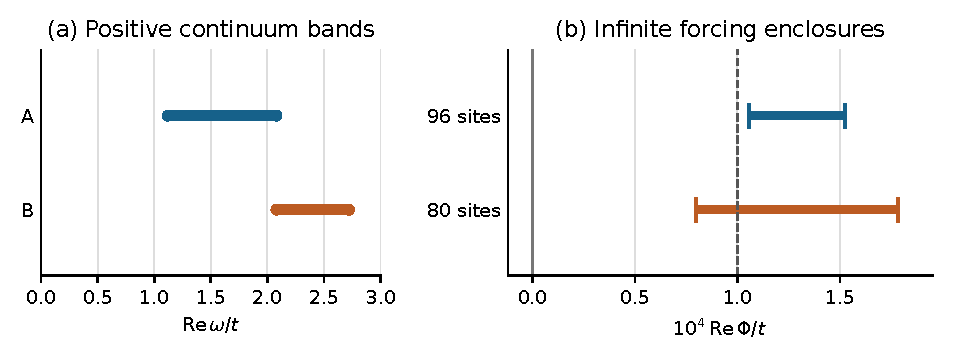
\includegraphics[width=\linewidth]{figures/certified-bounds.pdf}
\caption{Positive real parts of the one-particle continuum frequencies
(left) and certified enclosures of the same infinite on-shell forcing
(right). The intervals on the right include the inverse and infinite-tail
error; they are not statistical error bars. Both exclude zero, while only
the $96$-site witness proves $\Rea\Phi/t>10^{-4}$ (dashed line).
The half-line result is obtained from each complete error bound, not from
the apparent agreement of two finite approximations.}
\label{fig:bounds}
\end{figure}

The algebra and the boundary restoration admit separate checks. Exact
occupation-bit and Pauli matrices agree for $L=2,4,6$, including unequal
pairing and a nonzero chemical-potential control. The quartic source and
the physical parity agree in the original spin algebra. A deterministic
Gaussian-integer cubic test gives exact agreement of $156$ quintic
coefficients between direct Clifford multiplication and the determinant
contraction. Omitting the cutoff-crossing bond changes that test functional
by a nonzero amount of order $0.005t$, so it detects the relevant boundary
error. The small $L=16$ witness is inconclusive for the infinite functional;
its failure to exclude zero is not interpreted as evidence against the
larger certificate.

\section{Contradiction, operator domain and physical interpretation}
\label{sec:contradiction}
If an exponentially localized $Q_2$ satisfied~\eqref{eq:second}, project
that equation onto $A^3B^2$. The unique $Q_1$ has only the linear and cubic
parts already constructed, and the linear part cannot produce this
degree-five forcing. Thus the projected right-hand side is precisely
$-[V_4,Q_{1,\mathrm{cub}}]_{A^3B^2}$.

For an exponentially localized operator, its fixed-degree coefficient
tails are absolutely summable. Indeed, the number of degree-five monomials
with largest physical index $r$ grows only polynomially, whereas tracial
$L^2$ tails are bounded by the exponentially small operator-norm
approximation error. Cauchy--Schwarz gives summable $\ell^1$ shells.
The bounded left rows therefore define an absolutely convergent
functional, and finite-range summation by parts has no boundary term at
infinity. At the exact root of~\eqref{eq:resonance},
\begin{equation}
 \ell_5([H_0,Q_2]_{A^3B^2})=\Omega\ell_5((Q_2)_{A^3B^2})=0.
 \label{eq:contradiction}
\end{equation}
The right-hand side of~\eqref{eq:second}, however, has a nonzero
functional by~\eqref{eq:positive}. This contradiction proves the second
assertion of Proposition~\ref{prop:main}.

There is no hidden bounded-Hamiltonian assumption. If $h_j$ is a uniformly
bounded nearest-neighbour interaction and $Q$ satisfies~\eqref{eq:locality},
then, for large $j$, $[h_j,Q^{[j-1]}]=0$ and
$\norm{[h_j,Q]}\leq2\norm{h_j}C_Qe^{-\kappa_Q(j-1)}$.
The commutator series converges in norm. For a twice norm-differentiable
exact branch, pair its equation with an arbitrary local test operator
$T$ under the tracial bilinear pairing. Cyclicity gives
\begin{equation}
 \tau\bigl(T[H(\epsilon),Q(\epsilon)]\bigr)
       =-\tau\bigl([H(\epsilon),T]Q(\epsilon)\bigr).\label{eq:domain}
\end{equation}
The commutator on $T$ is a finite local sum, so the right-hand side is a
bounded functional of $Q(\epsilon)$ and can be differentiated twice.
The resulting coefficient equations hold against all local tests.
The norm convergence of the coefficient commutators then yields
Eqs.~\eqref{eq:first} and~\eqref{eq:second} as operator equations.
Differentiating the square normalization gives $\{Q_0,Q_1\}=0$.

The physical conclusion is a controlled failure of smooth, localized
edge-operator continuation even when each positive one-particle band is
separated from the imaginary axis and the first-order equation is regular.
The obstruction is a forced continuum channel at second order. This does
not assert that every finite-$\epsilon$ edge mode is absent. Nonanalytic
branches, branches with nonlocal derivatives, weak edge modes and
prethermal operators remain outside the statement. No lifetime, exceptional
point, finite-$\epsilon$ phase boundary, or many-body eigenvalue-pairing
theorem follows. In a non-normal problem, a small commutator alone would
not supply spectral conditioning or a conserved normalized expectation
value.

The comparison with uniform XYZ is also restricted. Bond alternation here
cannot be removed by a global spin-axis rotation or a common energy
rescaling. Fendley's uniform construction~\cite{Fendley2016} is not
contradicted; the discussion of spatially varying couplings there gives
low-order evidence, rather than an all-order result for the present point.
The finite boundary modification distinguished in the XYZ treatment of
Ref.~~\cite{Moudgalya2026}, Sec.~VI, is likewise different from the physical
half-line used here. Resonance-based boundary obstructions in
Ref.~~\cite{Olund2025} motivate the mechanism, but their Hermitian interface
models do not provide this complex on-shell forcing and its tail control.
These comparisons support a concrete restricted contribution, without an
exhaustive priority claim. The broader problem of finding an exact phase
boundary or exceptional-point condition away from the solvable Kitaev
slice remains unresolved.

\section*{Data and code availability}
The accompanying reproducibility files contain the two dyadic witnesses,
the independent certificate implementation, an isolated replay driver,
reference output records, and the script and data for
Fig.~\ref{fig:bounds}. The README specifies the environment and commands.
The numerical bounds support the analytic half-line argument given here;
finite computations alone do not prove spectral completeness or locality.

\section*{Acknowledgements and use of generative AI}
OpenAI Codex was used for literature assistance, formulation and analysis
of the restricted claim, symbolic and numerical code, internal verification,
and manuscript drafting. GPT-6 was used for manuscript preparation; the
complete model/version inventory for earlier phases remains to be confirmed.
The checks described here include separate AI-assisted implementations;
they are not external peer review.
Human scientific review, verification of every cited source, and critical
revision of the generated text remain pending for this local draft.
The author must confirm the complete tool/version disclosure and take
responsibility for the final work before any submission.

\appendix
\section{Exponential-weight inverse estimate}\label{app:weight}
With $r=|\rho|^2$, let $W_s q$ have components $e^{s(n-1)}q_n$.
Geometric sums give
\begin{align}
 N(s)^2&=\norm{W_sq}_2^2=\frac{|C|^2}{1-re^{2s}},\notag\\
 D(s)^2&=\norm{(W_s-\Id)q}_2^2
 =|C|^2\left[\frac1{1-re^{2s}}-\frac2{1-re^s}+\frac1{1-r}\right].
 \label{eq:geometric}
\end{align}
Conjugating the three nearest-neighbour factors changes their sum by at most
$2(|h_A|+2|h_B|)(e^\alpha-1)$. For the bilinear rank-one projector,
\begin{equation}
 \norm{W_\alpha P_0W_\alpha^{-1}-P_0}
 \leq D(\alpha)N(-\alpha)+N(0)D(-\alpha).
\end{equation}
Hence a valid value of $E$ in~\eqref{eq:weighted} is
\begin{equation}
 E=2(|h_A|+2|h_B|)(e^\alpha-1)
       +8[D(\alpha)N(-\alpha)+N(0)D(-\alpha)].
\end{equation}
Using~\eqref{eq:inverse}, the weighted inverse is bounded by $M/(1-ME)$.
The enclosed values are $M<33.317951$, $ME<0.454720583$, and
$M/(1-ME)<61.102528$. These bounds concern a fixed Clifford degree and a
specified exponential weight, with no all-degree norm estimate assumed.

\section{Enclosure of the two-coordinate resonance}\label{app:root}
The exact decimal center is
\begin{align*}
 x_c&=\texttt{0.914005998943111754560338502271033241599810017455941304810241},\\
 y_c&=\texttt{-0.769581730425783703625420540788997375179263443033756807855182}.
\end{align*}
Let $F=(\Rea\Omega,\Ima\Omega)$ and $B_c$ be the real infinity-norm
box with this center and radius $r_c=10^{-20}$. The checker constructs an
exact dyadic matrix $C_0$ by rounding the inverse central Jacobian to binary
floating point, then interpreting each entry as its exact binary rational.
All following evaluations use ball arithmetic. It verifies $C_0$ is
nonsingular and obtains
\begin{equation}
 \norm{C_0F(x_c,y_c)}_\infty<3.257\times10^{-61},\qquad
 \sup_{B_c}\norm{\Id-C_0DF}_\infty<2.762\times10^{-16}.\label{eq:rootbounds}
\end{equation}
Thus $z\mapsto z-C_0F(z)$ maps $B_c$ into itself and is a contraction,
because the first bound plus $r_c$ times the second is less than $r_c$.
Its fixed point is a zero of $F$. The differentiations are explicit:
\begin{equation}
 \partial_x\Omega=\frac{4p_Ah_A}{\omega_A(x)},\qquad
 \partial_y\Omega=-4p_Bh_B\left[
       \frac1{\omega_B(y-1/100)}+\frac1{\omega_B(y+1/100)}\right],
\end{equation}
where $\omega_s(x)=2\sqrt{p_s^2+h_s^2+2p_sh_sx}$ in this appendix.
The supplied code records $C_0$ and evaluates the left rows over the entire
box. The approximate decimal center in the main text is not the certificate
input.

\section{Residual and determinant contraction}\label{app:residual}
Use zero-based physical indices in this appendix, so
$m_j=6/5$ for even $j$ and $4/5$ for odd $j$.
Write a cubic vector as $X=\sum_{i,b<c}X_{i,bc}A_iB_bB_c$ and extend
$X_{i,cb}=-X_{i,bc}$. For the $L$-site witness the array shape is
$(L-1,L,L)$. It is embedded into $(L,L+1,L+1)$ before applying the
nearest-neighbour commutator. This includes every link that acts on its
support. After a common power-of-two denominator is extracted from the
binary coefficients, the rational quadratic action is performed with
unbounded Gaussian integers. The geometric forcing and normalization are
then enclosed with balls.

Let $r_{\rm fin}$ be the coefficient $\ell^2$ residual of the restored
physical action with its explicitly represented source terms, and
$Z_{bc}=\sum_n C\rho^n X_{2n,bc}$. Triangle inequalities give
\begin{equation}
 \norm{W_\alpha R}_2\leq
 e^{3\alpha(N+1)}r_{\rm fin}+T_N
 +8N(\alpha)e^{2\alpha(N+1)}\norm{Z}_2,\qquad N=L/2.
 \label{eq:residualformula}
\end{equation}
The finite weights deliberately overestimate every represented output
index. $T_N$ in~\eqref{eq:tail} covers the entire complement, so changing
which of the last geometric source entries is explicitly represented does
not change the logical coverage of the bound. The normalization term is
necessary even when a numerical solve intended to enforce $P_{0,A}X=0$.

For clarity, the finite functional can be evaluated without assembling a
five-index tensor. Let $a_j$ be the column of the three $A$ rows at site
$j$, and let $b_s(j)$ be the $s$th $B$ row. With
$T_i(j,s)=\sum_r X_{i,jr}b_s(r)$, define $k=j+1$ and obtain directly from
Eq.~\eqref{eq:v4}
\begin{align}
 \Phi(X)=\sum_{i=0}^{L-2}\sum_{j=0}^{L-1}m_j\det(a_j,a_k,a_i)
 \bigl[&b_1(k)T_i(j,2)-b_2(k)T_i(j,1)\notag\\
       &-b_1(j)T_i(k,2)+b_2(j)T_i(k,1)\bigr].\label{eq:contraction}
\end{align}
The $T_i(k,s)$ terms vanish for $k=L$ by zero extension. The
$j=L-1$ summand is retained: it is the quartic bond crossing the finite
support. Direct Clifford multiplication checks the sign and ordering in
Eq.~\eqref{eq:contraction} independently.

The $96$-site witness comes from a finite spectral solve with residual
correction; the $80$-site witness was generated independently by GMRES from
zero. Both are checked by the Gaussian-integer and ball-arithmetic route
above. New witnesses, which the supplied checker can generate, require
recertification: neither solver tolerances nor matching decimal digits
replace Eq.~\eqref{eq:residualformula}.

\begingroup
\small
\setlength{\bibsep}{5pt}
\bibliographystyle{unsrtnat}
\bibliography{references}
\endgroup
\end{document}
